%!TEX root=../document.tex

\section{What is E-Sport?}
The eSports, also known as electronic sports, competitive gaming, professional gaming, or pro gaming, is a form of competition that is facilitated by electronic systems, particularly video games. The input of players and teams as well as the output of the eSports system are mediated by human-computer interfaces. Most commonly, eSports take the form of organized, multiplayer video game competitions, particularly between professional players. The most common video game genres associated with eSports are real-time strategy, fighting, first-person shooter (FPS), and multiplayer online battle arena (MOBA). Tournaments such as The International, the League of Legends World Championship, the Battle.net World Championship Series, the Evolution Championship Series, the Intel Extreme Masters, and the Smite World Championship provide live broadcasts of the competition, and prize money and salaries to competitors.

Although organized online and offline competitions have long been a part of video game culture, participation and spectatorship of such events have seen a large surge in popularity from the late 2000s and early 2010s. While competitions around 2000 were largely between amateurs, the proliferation of professional competitions and growing viewership now supports a significant number of professional players and teams, and many video game developers now build features into their games designed to facilitate such competition.

The genre of fighting games and arcade game fighters have also been popular in amateur tournaments, although the fighting game community has often distanced themselves from the eSports label. In the mid 2010s, the most successful titles featured in professional competition were the multiplayer online battle arena (MOBA) games Dota 2 and League of Legends, and the first person shooter game Counter-Strike: Global Offensive. Other games with significant earnings include Smite, StarCraft II, Call of Duty, Heroes of the Storm, Hearthstone and Overwatch.

\begin{figure}[!h]
	\begin{center}
		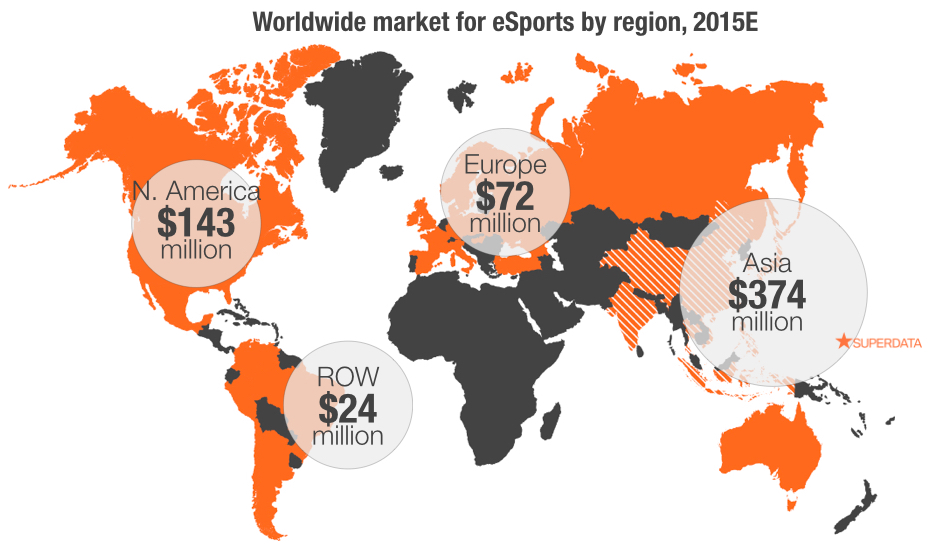
\includegraphics[width=0.68\linewidth]{images/esport_market}
		\caption{Earnings by region \url{http://s3-eu-west-1.amazonaws.com/cdx-website-wp-media/wp-content/uploads/20160727010807/Worldwide-eSports-market-size-2015.jpg}}
	\end{center}
\end{figure}
\newpage

South Korea has the several established eSports organizations, which have licensed pro gamers since the year 2000. Recognition of eSports competitions outside South Korea has come somewhat slower. Along with South Korea, most competitions take place in Europe, North America and China. Despite its large video game market, eSports in Japan is relatively underdeveloped, which has been attributed largely to its broad anti-gambling laws.



In 2013, it was estimated that approximately 71.5 million people worldwide watched eSports. The increasing availability of online streaming media platforms, particularly Twitch.tv, has become central to the growth and promotion of eSports competitions. Demographically, Major League Gaming has reported viewership that is approximately 85\% male and 15\% female, with 60\% of viewers between the ages of 18 and 34.
The global eSports market generated US \$325 million of revenue in 2015 and is expected to make \$493 million in 2016; the global eSports audience in 2015 was 226 million people.

\section{History}
	\subsection{Roots 1972-1994}
		
		The earliest known video game competition took place on 19 October 1972 at Stanford University for the game Spacewar. Stanford students were invited to an "Intergalactic spacewar olympics" whose grand prize was a year's subscription for Rolling Stone, with Bruce Baumgart winning the five-man-free-for-all tournament and Tovar and Robert E. Maas winning the Team Competition. The Space Invaders Championship held by Atari in 1980 was the earliest large scale video game competition, attracting more than 10,000 participants across the United States, establishing competitive gaming as a mainstream hobby.
		
		In the summer of 1980, Walter Day founded a high score record keeping organization called Twin Galaxies. The organization went on to help promote video games and publicize its records through publications such as the Guinness Book of World Records, and in 1983 it created the U.S. National Video Game Team. The team was involved in competitions, such as running the Video Game Masters Tournament for Guinness World Records and sponsoring the North American Video Game Challenge tournament.
		
		During the 1970s and 1980s, video game players and tournaments begun being featured in popular websites and magazines including Life and Time. One of the most well known classic arcade game players is Billy Mitchell, for his listing as holding the records for high scores in six games including Pac-Man and Donkey Kong in the 1985 issue of the Guinness Book of World Records. Televised eSports events aired during this period included the American show Starcade which ran between 1982 and 1984 airing a total of 133 episodes, on which contestants would attempt to beat each other's high scores on an arcade game. A video game tournament was included as part of TV show That's Incredible!, and tournaments were also featured as part of the plot of various films.
		\newpage
	\subsection{Networkbased E-Sport 1995-1999}
	
		In the 1990s, many games benefited from increasing internet connectivity, especially PC games. For example, the 1988 game Netrek was an Internet game for up to 16 players, written almost entirely in cross-platform open source software. Netrek was the third Internet game, the first Internet game to use metaservers to locate open game servers, and the first to have persistent user information. In 1993 it was credited by Wired Magazine as "the first online sports game".
		
		Large eSports tournaments in the 1990s include the 1990 Nintendo World Championships, which toured across the United States, and held its finals at Universal Studios Hollywood in California. Nintendo held a 2nd World Championships in 1994 for the Super Nintendo Entertainment System called the Nintendo PowerFest '94. There were 132 finalists that played in the finals in San Diego, California. Mike Iarossi took home 1st prize. Blockbuster Video also ran their own World Game Championships in the early 1990s, co-hosted by GamePro magazine. Citizens from the United States, Canada, the United Kingdom, Australia, and Chile were eligible to compete. Games from the 1994 championships included NBA Jam and Virtua Racing.
		
		Television shows featuring eSports during this period included the British shows GamesMaster and Bad Influence! the Australian gameshow Amazing, which would show two children competing in various Nintendo games in order to win points.
		
		Tournaments established in the late 1990s include the Cyberathlete Professional League (CPL), QuakeCon, and the Professional Gamers League. PC games played at the CPL included the Counter-Strike series, Quake series, and Warcraft.
		
		\begin{figure}[!h]
			\begin{center}
				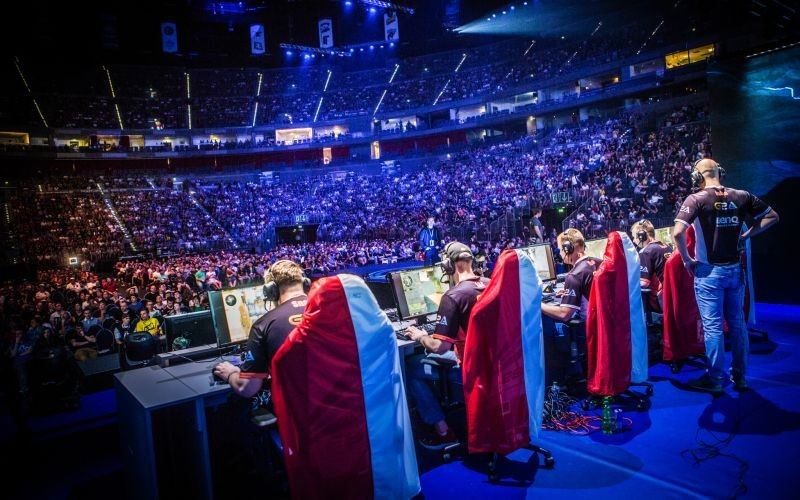
\includegraphics[width=0.68\linewidth]{images/esports_csgo}
				\caption{Counter Strike Global Offensive Tournament 2015}
			\end{center}
		\end{figure}
		\newpage
	\subsection{Global Tournaments}
		
		The growth of eSports in South Korea is thought to have been influenced by the mass building of broadband internet networks following the 1997 Asian financial crisis. It is also thought that the high unemployment rate at the time caused many people to look for things to do while out of work. Instrumental to this growth of eSports in South Korea was the prevalence of the Komany-style internet cafe/LAN gaming center, known as a PC bang. The Korean e-Sports Association, an arm of the Ministry of Culture, Sports and Tourism, was founded in 2000 to promote and regulate eSports in the country.
		
		In the second decade of the 21st century, eSports has grown tremendously, incurring a large increase in both viewership and prize money. Although large tournaments were founded before the 21st century, the number and scope of tournaments has increased significantly, going from about 10 tournaments in 2000 to about 260 in 2010. Many successful tournaments were founded during this period, including the World Cyber Games, the Intel Extreme Masters, and Major League Gaming. The proliferation of tournaments included experimentation with competitions outside traditional eSports genres. For example, the September 2006 FUN Technologies Worldwide Webgames Championship featured 71 contestants competing in casual games for a \$1 million grand prize.
		
		In April 2006 the G7 teams federation were formed by seven prominent Counter-Strike teams. The goal of the organization was to increase stability in the eSports world, particularly in standardizing player transfers and working with leagues and organizations. The founding members were 4 Kings, Fnatic, Made in Brazil, Mousesports, NiP, SK-Gaming, Team 3D. The organization only lasted until 2009 before dissolving.
		
								\begin{figure}[!h]
									\begin{center}
										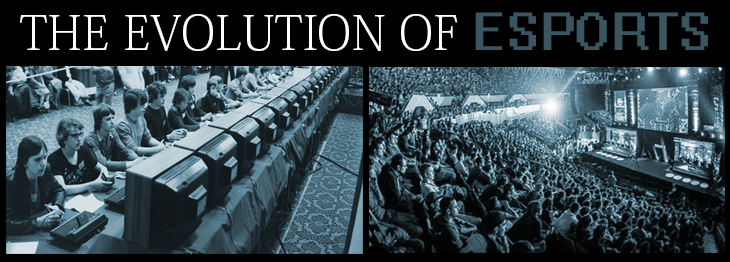
\includegraphics[width=0.68\linewidth]{images/evolution}
										\caption{The evolution of E-Sports}
									\end{center}
								\end{figure}
		
		The 2000s was also the peak of televised eSports. Television coverage was best established in South Korea, with StarCraft and Warcraft III competitions regularly televised by dedicated 24-hour cable TV game channels Ongamenet and MBCGame. Elsewhere, eSports television coverage was sporadic. The German GIGA Television covered eSports until its shutdown in 2009. The United Kingdom satellite television channel XLEAGUE.TV broadcast eSports competitions from 2007 to 2009. The online eSports only channel ESL TV briefly attempted a paid television model re-named GIGA II from June 2006 to autumn 2007. The French channel Game One broadcast eSports matches in a show called Arena Online for the Xfire Trophy. The United States channel ESPN hosted Madden NFL competitions in a show called Madden Nation from 2005 to 2008. DirectTV broadcast the Championship Gaming Series tournament for two seasons in 2007 and 2008. CBS aired prerecorded footage of the 2007 World Series of Video Games tournament that was held in Louisville, Kentucky, US. The G4 television channel originally covered video games exclusively, but broadened its scope to cover technology and men's lifestyle, though has now shutdown.
		

		
		The popularity and emergence of online streaming services have helped the growth of eSports in this period, and are the most common method of watching tournaments. Twitch, an online streaming platform launched in 2011, routinely streams popular eSports competitions. In 2013, viewers of the platform watched 12 billion minutes of video on the service, with the two most popular Twitch broadcasters being League of Legends and Dota 2. During one day of The International, Twitch recorded 4.5 million unique views, with each viewer watching for an average of two hours.
		
		The modern eSports boom has also seen a rise in video games companies embracing the eSports potential of their products. After many years of ignoring and at times suppressing the eSports scene, Nintendo hosted Wii Games Summer 2010. Spanning over a month, the tournament had over 400,000 participants, making it the largest and most expansive tournament in the company's history. In 2014 Nintendo hosted an invitational Super Smash Bros. for Wii U competitive tournament at the 2014 Electronic Entertainment Expo (E3) press conference that was streamed online on Twitch. Halo developers 343 Industries announced in 2014 plans to revive Halo as an eSport with the creation of the Halo Championship Series and a prize pool of \$50,000 USD. Both Blizzard Entertainment and Riot Games have their own collegiate outreach programs with their North American Collegiate Championship. Since 2013 universities and colleges in the United States such as Robert Morris University Illinois and the University of Pikeville have recognized eSports players as varsity level athletes and offer athletic scholarships.
		
		In 2014, the largest independent eSports league, Electronic Sports League, partnered with the local brand Japan Competitive Gaming to try and grow eSports in the country.
		
		Physical viewership of eSports competitions and the scope of events have increased in tandem with the growth of online viewership. In 2013 the Season 3 League of Legends World Championship was held in a sold-out Staples Center. The 2014 League of Legends World Championship in Seoul, South Korea had over 40,000 fans in attendance and featured the band Imagine Dragons, and opening and closing ceremonies in addition to the competition.
	
		\newpage
\section{Classification as a sport}
		Labeling video games as sports is somewhat controversial. While some point to the growth in popularity of eSports as justification for designating some games as sports, others contend that video games will never reach the status of "true sports". However popularity is not the only reason identified: some have argued that "careful planning, precise timing, and skillful execution" Tought to be what classifies an activity as sport, and that physical exertion and outdoor playing areas are not required by all traditional or non-traditional 'sports'. In a 2014 technology conference, when asked about the recent buyout of popular game streaming service Twitch, ESPN president John Skipper described eSports as "\textit{not a sport – [they're] a competition.}". In addition, many in the fighting games community maintain a distinction between their competitive gaming competitions and the more commercially connected eSports competitions of other genres. Video games are sometimes classified as a mind sport. In the 2015 eSports World Championship hosted by the International e-Sports Federation, an eSports panel was hosted with guests from international sports society to discuss the future recognition of eSports as a recognized, legitimate sporting activity worldwide.
		
				\begin{figure}[!h]
					\begin{center}
						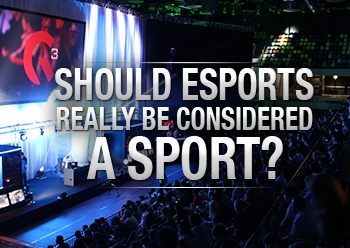
\includegraphics[width=0.68\linewidth]{images/is_esport_sport}
						\caption{Is E-Sports really a sport?}
					\end{center}
				\end{figure}
\section{Games}
	A number of games are popular among professional competitors. The tournaments which emerged in the mid-1990s coincided with the popularity of fighting games and first-person shooters, genres which still maintain a devoted fan base. In the 2000s, real-time strategy games became overwhelmingly popular in South Korean internet cafés, with crucial influence on the development of eSports worldwide. After 2010 with the release of the Warcraft III: The Frozen Throne mod Defense of the Ancients, multiplayer online battle arena games became popular as eSports. Competitions exist for many titles and genres, though currently the most popular games are Counter-Strike: Global Offensive, Call of Duty, League of Legends, Dota 2, Smite, Rocket League, World of Tanks, Heroes of the Storm, Hearthstone: Heroes of Warcraft, Super Smash Bros. Melee and StarCraft II. Hearthstone has also popularized the digital collectible card game genre since its release in 2014.

\section{Types of Video game design}
	While it is common for video games to be designed with the experience of the player in game being the only priority, many successful eSports games have been designed to be played professionally from the beginning. Developers may decide to add dedicated eSports features, or even make design compromises to support high level competition. Games such as StarCraft II, League of Legends, and Dota 2 have all been designed, at least in part, to support professional competition.
	\subsection{Spectator mode}
		In addition to allowing players to participate in a given game, many game developers have added dedicated observing features for the benefit of spectators. This can range from simply allowing players to watch the game unfold from the competing player's point of view, to a highly modified interface that gives spectators access to information even the players may not have. The state of the game viewed through this mode may tend to be delayed by a certain amount of time in order to prevent either teams in a game from gaining a competitive advantage.
	\subsection{Online}
		A very common method for connection is the Internet. Game servers are often separated by region, but high quality connections allow players to set up real-time connections across the world. Downsides to online connections include increased difficulty detecting cheating compared to physical events, and greater network latency, which can negatively impact players' performance, especially at high levels of competition. Many competitions take place online, especially for smaller tournaments and exhibition games.
	\subsection{Local area network}
		Additionally, competitions are also often conducted over a local area network or LAN. The smaller network usually has very little lag and higher quality. Because competitors must be physically present, LANs help ensure fair play by allowing direct scrutiny of competitors. This helps prevent many forms of cheating, such as unauthorized hardware or software modding. The physical presence of competitors helps create a more social atmosphere at LAN events. Many gamers organize LAN parties or visit Internet cafés, and most major tournaments are conducted over LANs.
		
		\newpage
\section{Tournaments}
		eSports tournaments are almost always physical events in which occur in front of a live audience. The tournament may be part of a larger gathering, such as Dreamhack, or the competition may be the entirety of the event, like the World Cyber Games. Competitions take several formats, but the most common are single or double elimination, sometimes hybridized with group stage. Competitions usually have referees or officials to monitor for cheating.
		
		Although competitions involving video games have long existed, eSports underwent a significant transition in the late 1990s. Beginning with the Cyberathlete Professional League in 1997, tournaments became much larger, and corporate sponsorship became more common. Increasing viewership both in person and online brought eSports to a wider audience. Major tournaments include the World Cyber Games, the North American Major League Gaming league, the France based Electronic Sports World Cup, and the World e-Sports Games held in Hangzhou, China.
		
		For well established games, total prize money can amount to millions of U.S. dollars a year. As of 10 September 2016, Dota 2 has awarded approximately US\$86 million in prize money within 632 registered tournaments, with 23 players winning over \$1 million. League of Legends awarded approximately \$30 million within 1749 registered tournaments, but in addition to the prize money, Riot Games provides salaries for players within their League of Legends Championship Series. Nonetheless, there has been criticism to how these salaries are distributed, since most players earn a fairly low wage but a few top players have a significantly higher salary, skewing the average earning per player.
		
		Often, game developers provide prize money for tournament competition directly, but sponsorship may also come from third parties, typically companies selling computer hardware, energy drinks, or computer software. Generally, hosting a large eSports event is not profitable as a stand alone venture. For example, Riot has stated that their headline League of Legends Championship Series is "a significant investment that we're not making money from".
\section{Teams and associations}
		Professional gamers are often associated with gaming teams and broader gaming associations. Teams like OpTic Gaming, Evil Geniuses, Team SoloMid, Cloud9, Fnatic, Mineski, Counter Logic Gaming, SK Telecom T1, Splyce, EnVyUs, and Natus Vincere consist of several professionals. In addition to prize money from tournament wins, players may also be paid a separate team salary. Team sponsorship may cover tournament travel expenses or gaming hardware. Prominent eSports sponsors include companies such as Logitech and Razer. Teams feature these sponsors on their website, team jerseys and on their social media, in 2016 the biggest teams have social media followings of over 1.27 million.
		
		Traditional sports athletes have shown interest in eSports, examples being Rick Fox's ownership of Echo Fox and Shaquille O'Neal's investment in NRG eSports. Some soccer teams, such as Schalke 04 in Germany and PSG eSports in France, have ownership in eSports teams
\section{Ethics}
	\subsection{Performance-enhancing drugs}
	Reports of widespread use of performance-enhancing drugs in eSports are not uncommon, with players discussing their own, their teammates' and their competitors' use and officials acknowledging the prevalence of the issue. Players often turn to stimulants such as Ritalin, Adderall and Vyvanse, drugs which can significantly boost concentration, improve reaction time and prevent fatigue. Selegiline, a drug used to treat Parkinson's disease, is reportedly popular because, like stimulants, it enhances mood and motivation. Conversely, drugs with calming effects are also sought after. Some players take propanolol, which blocks the effects of adrenaline, or Valium, which is prescribed to treat anxiety disorder, in order to remain calm under pressure.
	\subsection{Player exploitation}
	There has been some concern over the quality of life and potential mistreatment of players by organizations, especially in South Korea. Korean organizations have been accused of refusing to pay competitive salaries, leading to a slow exodus of Korean players to other markets. In an interview, League of Legends player Bae "Dade" Eo-jin said that "Korean players wake up at 1pm and play until 5am", and suggested that the 16 hour play schedule was a significant factor in causing burnout. Concerns over the mental health of players intensified in 2014 when League of Legends player Cheon "Promise" Min-Ki attempted suicide a week after admitting to match fixing.
	\subsection{Economics}
	League of Legends Championship Series and League of Legends Champions Korea offer guaranteed salaries for players. Despite this, online streaming is preferred by some players, as it is in some cases more profitable than competing with a team and streamers have the ability to determine their own schedule. The International tournament awards US\$10 million to the winners, however teams that do not have the same amount of success often do not have financial stability and frequently break up after failing to win.
	
	In 2015 it was estimated by SuperData Research that the global eSports industry generated revenue of around US\$748.8 million that year. Asia is the leading eSports market with over \$321 million in revenue, North America is around \$224 million, and Europe has \$172 million and the rest of the world for about \$29 million. Global eSports revenue is estimated to reach \textbf{\$1.9 billion by 2018.}
	\newpage
\section{Media coverage}
	\subsection{News reporting}
	The main medium for eSports coverage is the Internet. Coverage of eSports by general news organizations is generally sparse. Most reports come from news organizations with a technology or video games focus. Esports Heaven, RankR eSports, Esports Nation, and ESFI World are among the few independent news organizations specifically dedicated to eSports. Other typical sources for information include video game developer's websites, websites of professional teams, and independent community websites. However, in the mid-2010s, mainstream sports and news reporting websites, such as ESPN, Yahoo!, Sport1, Kicker, and Aftonbladet started dedicated eSports coverage.
	\subsection{Internet live streaming}
	Many eSports events are streamed online to viewers over the internet. With the shutdown of the Own3d streaming service in 2013, Twitch is by far the most popular streaming service for eSports, competing against other providers such as Hitbox.tv, Azubu, and YouTube Gaming. Dreamhack Winter 2011 reached 1.7 million unique viewers on Twitch. While coverage of live events usually brings in the largest viewership counts, the recent popularization of streaming services has allowed individuals to broadcast their own gameplay independent of such events as well. Individual broadcasters can enter an agreement with Twitch or hitbox in which they receive a portion of the advertisement revenue from commercials which run on the stream they create.
	
		\begin{figure}[!h]
			\begin{center}
				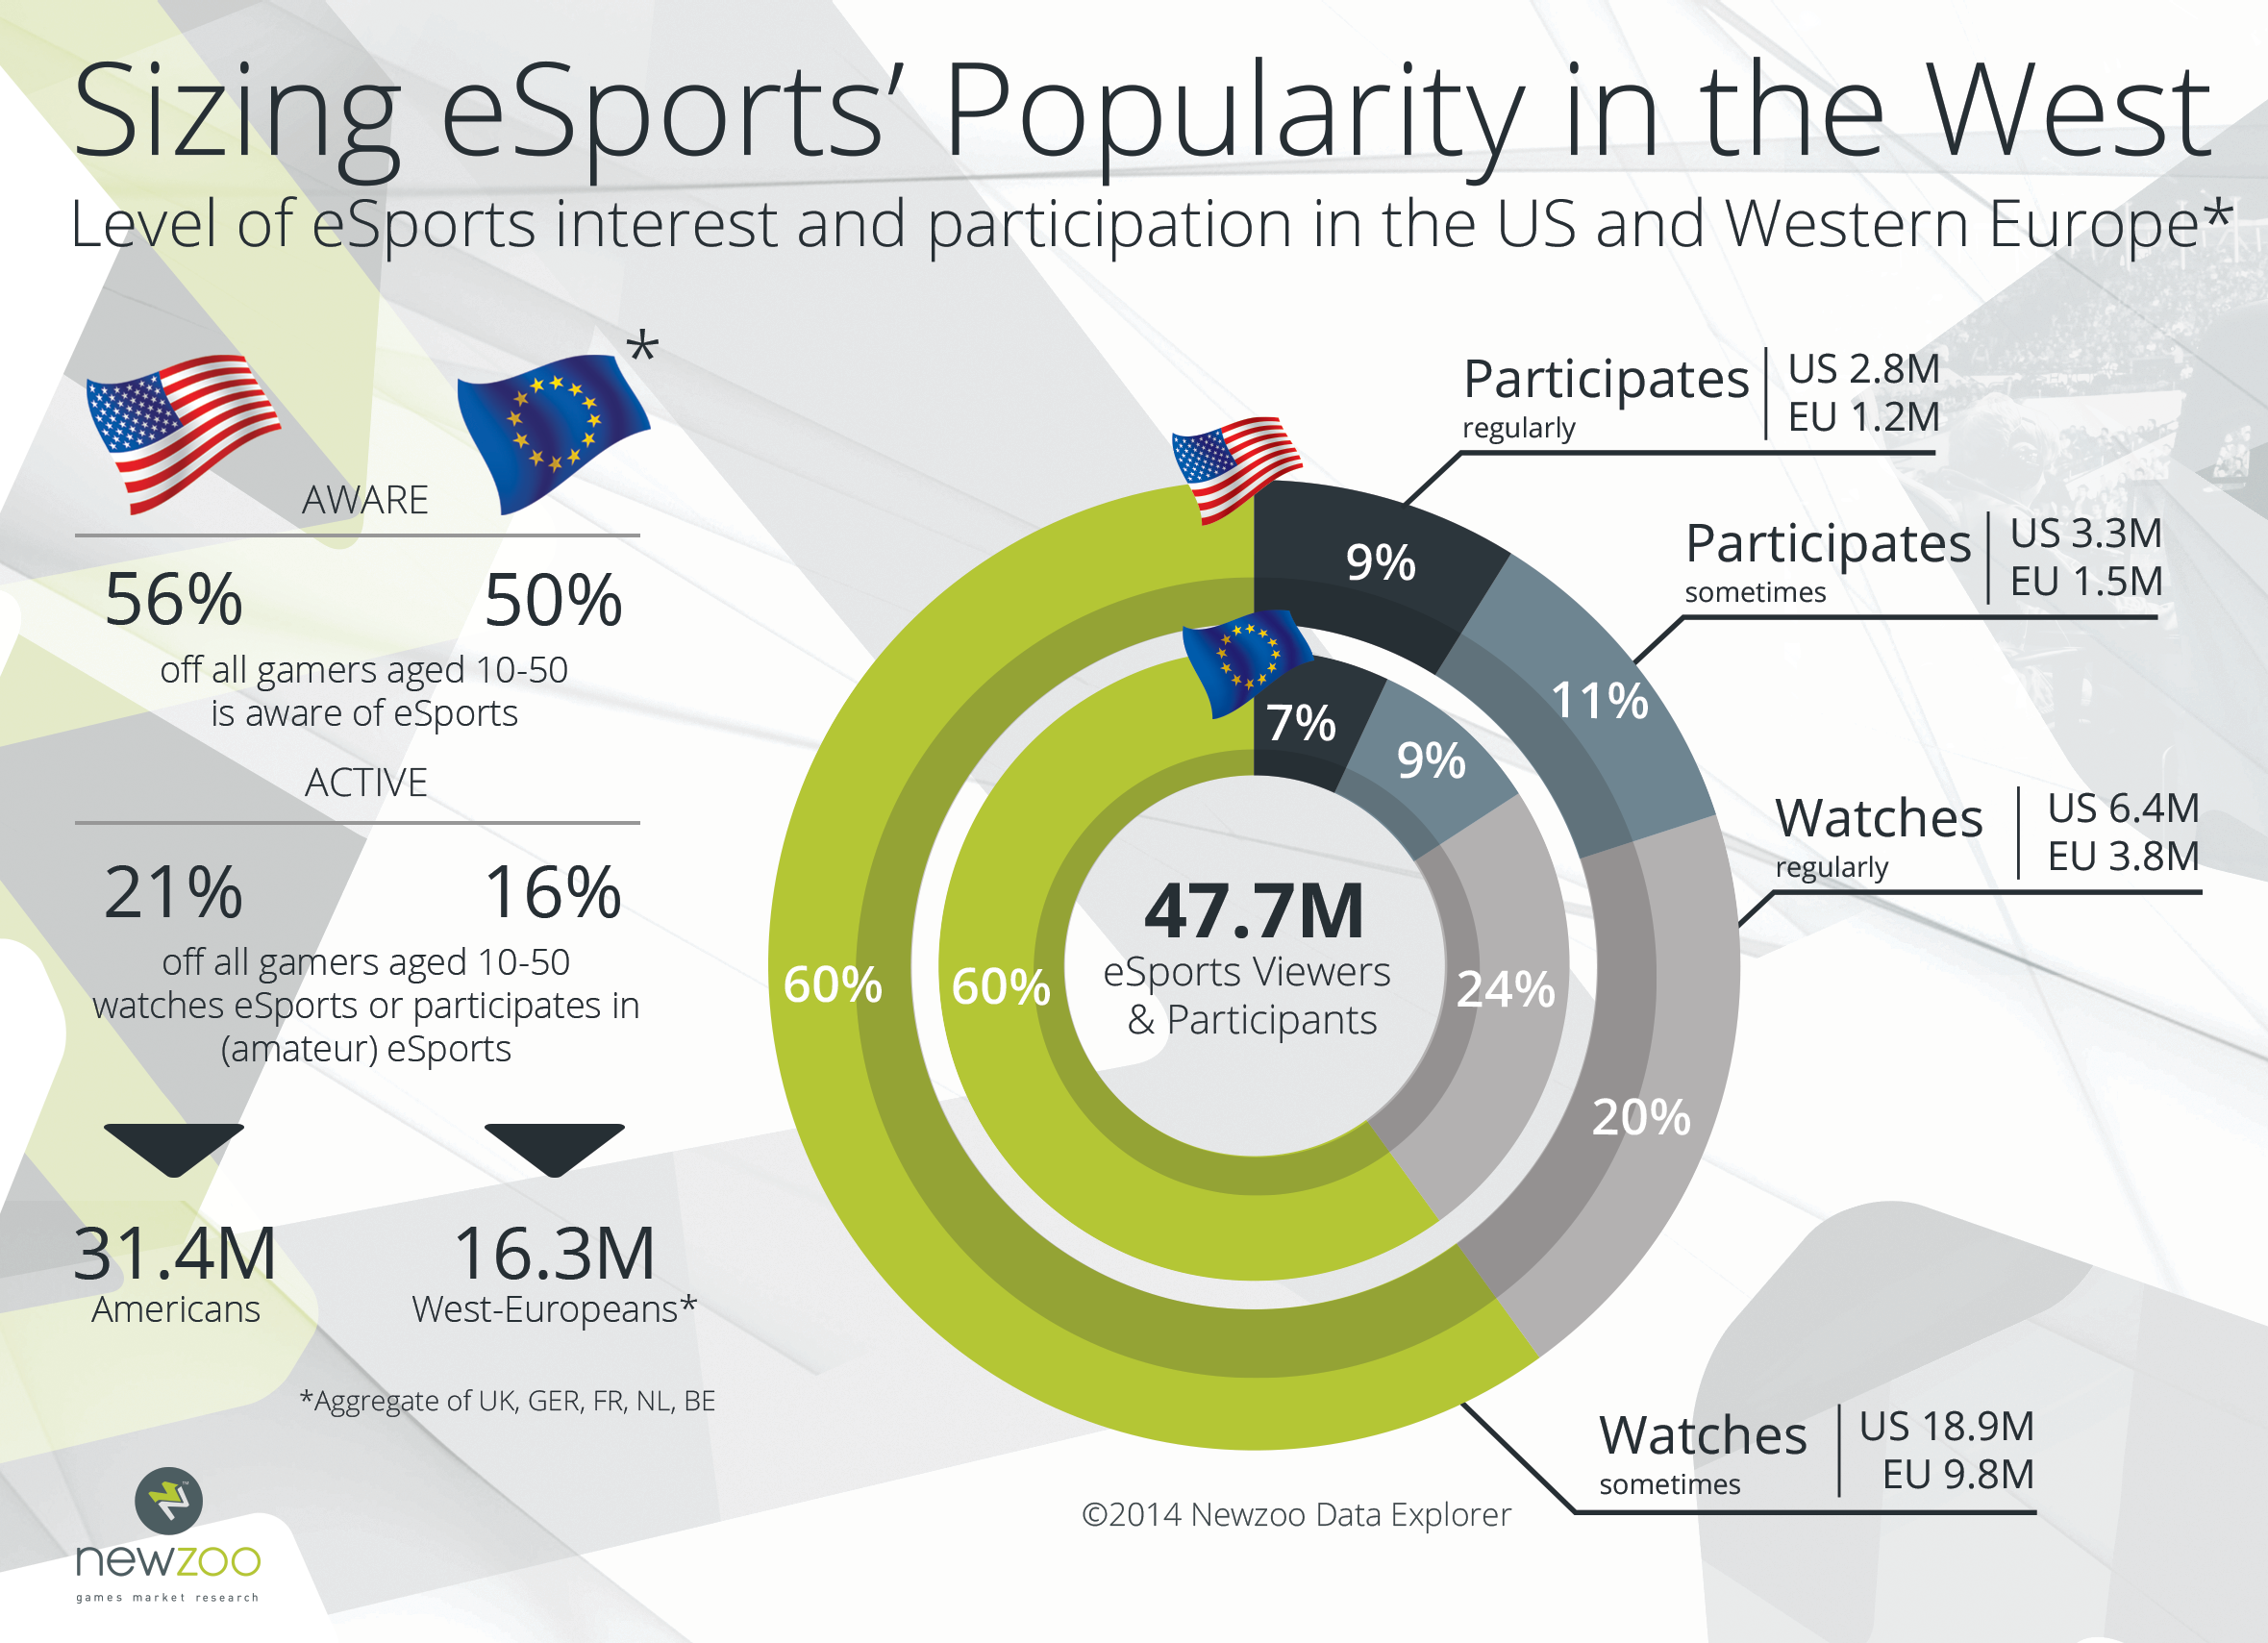
\includegraphics[width=0.8\linewidth]{images/newzoo_esport}
				\caption{E-Sports popularity in the West by \url{https://newzoo.com/wp-content/uploads/2014/04/Newzoo_eSports_Market_US-EU.png}}
			\end{center}
		\end{figure}
	\newpage
	
	\subsection{Television}
	Especially since the popularization of streaming in eSports, organizations no longer prioritize television coverage, preferring online streaming websites such as Twitch. Ongamenet continues to broadcast as an eSports channel in South Korea, but MBCGame was taken off the air in 2012. Riot Games' Dustin Beck stated that "TV's not a priority or a goal", and DreamHack's Tomas Hermansson said "eSports have a proven record to be successful on internet streaming only."
	
	On the night before the finals of The International 2014 in August, ESPN3 broadcast a half-hour special profiling the tournament. In 2015, ESPN2 broadcast Heroes of the Dorm, the grand finals of the Heroes of the Storm collegiate tournament. The first-place team from the University of California, Berkeley received tuition for each of the teams players, paid for by Blizzard and Tespa. The top four teams won gaming equipment and new computers. This was the first time an eSport had ever been broadcast on a major American television network. The broadcast was an attempt to broaden the appeal of eSports by reaching viewers who would not normally come across it. However, the broadcast was met with a few complaints. Those living outside of the United States were unable to view the tournament. Additionally, the tournament could not be viewed online via streams, cutting off a large portion of viewers from the main demographic in the process.
	
				
